\begin{figure}[htbp]
\centering
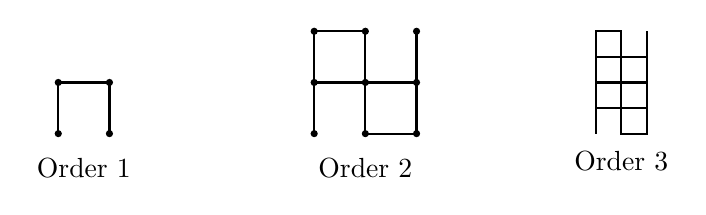
\begin{tikzpicture}[scale=0.65]
  \begin{scope}[xshift=-5cm]
    \draw[thick] (0,0)--(0,1)--(1,1)--(1,0);
    \foreach \x/\y in {0/0,0/1,1/1,1/0} {\fill (\x,\y) circle (2pt);}
    \node[below] at (0.5,-0.3) {Order 1};
  \end{scope}
  \begin{scope}[xshift=0cm]
    \draw[thick] (0,0)--(0,2)--(1,2)--(1,1)--(0,1)--(0,2) (1,1)--(2,1)--(2,2) (2,1)--(2,0)--(1,0)--(1,1);
    \foreach \x/\y in {0/0,0/1,0/2,1/2,1/1,2/1,2/2,2/0,1/0} {\fill (\x,\y) circle (2pt);}
    \node[below] at (1,-0.3) {Order 2};
  \end{scope}
  \begin{scope}[xshift=5.5cm,scale=0.5]
    \draw[thick] (0,0)--(0,4)--(1,4)--(1,3)--(0,3)--(0,4) (1,3)--(2,3)--(2,4) (2,3)--(2,2)--(1,2)--(1,3) (1,2)--(0,2)--(0,3) (0,2)--(0,1)--(1,1)--(1,2) (1,1)--(2,1)--(2,2) (2,1)--(2,0)--(1,0)--(1,1);
    \node[below] at (1,-0.3) {Order 3};
  \end{scope}
\end{tikzpicture}
\caption{Hilbert curve construction: each order recursively places four rotated copies in a U-shaped pattern.}
\label{fig:hilbert_curve}
\end{figure}
